\chapter{Функционал пользователя группы <<авторизованный пользователь>>.}

    См. \gloss{auth_user} в глоссарии.

    \section{Общие элементы страниц}
        \subsection{Главное меню}
            
            См. рис. \ref{fig:auth_main_menu}

            Все то же, что у неавторизованного пользователя (см.\ref{
                ec:baseitems_main_meu}), плюс пункт <<профиль пользователя>> со
                следующими элементами: 
            \begin{enumerate}
                \item ФИО пользователя.
                \item Количество баллов.
            \end{enumerate}


        \begin{figure}
            \center
            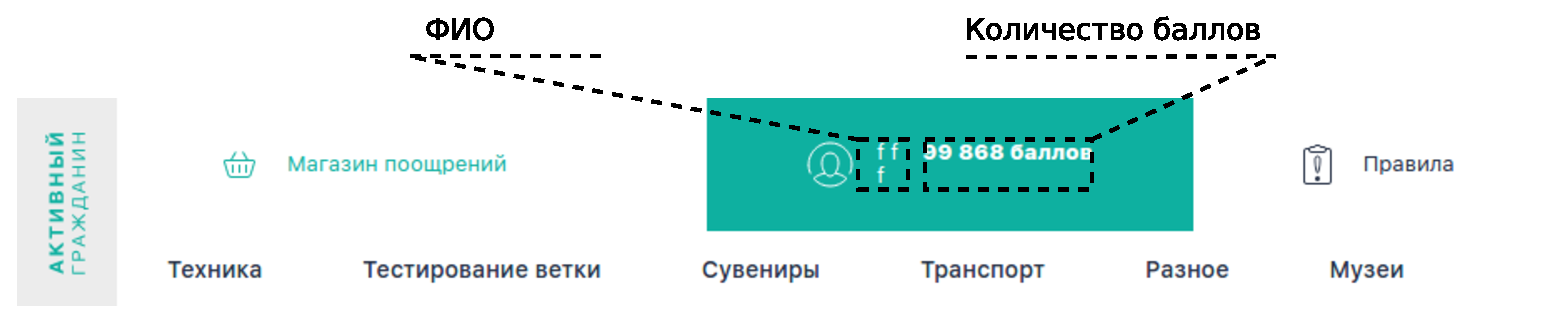
\includegraphics[width=170mm]{04_auth_funcs/figures/01.eps}
            \caption{Главное меню авторизованного пользователя}
            \label{fig:auth_main_menu}
        \end{figure}
        
        \subsection{Фильтр по цене и интересам}

            См. рис. \ref{fig:auth_filter}

            Вместо ссылки на авторизацию (см. 
            \ref{sec:noauth_filter_points}) появляется дополнительная вкладка
            <<у меня N баллов>>, задающая диапазон фильтрации товаров по 
            баллам.
            
            \begin{enumerate}
                \item По умолчанию выставляется число баллов от нуля до 
                количества, которое есть у пользователя.
                \item Есть элемент, позволяющий фильтровать товары 
                независимо от количества баллов у пользователя <<все баллы>>.
                \item Остальные элементы управления задают диапазоны между 
                порядками цен (0$\dots$10, 11$\dots$100 и т.д.).
                \item Выбрать можно только один диапазон.
            \end{enumerate}

            
            \begin{figure}
                \center
                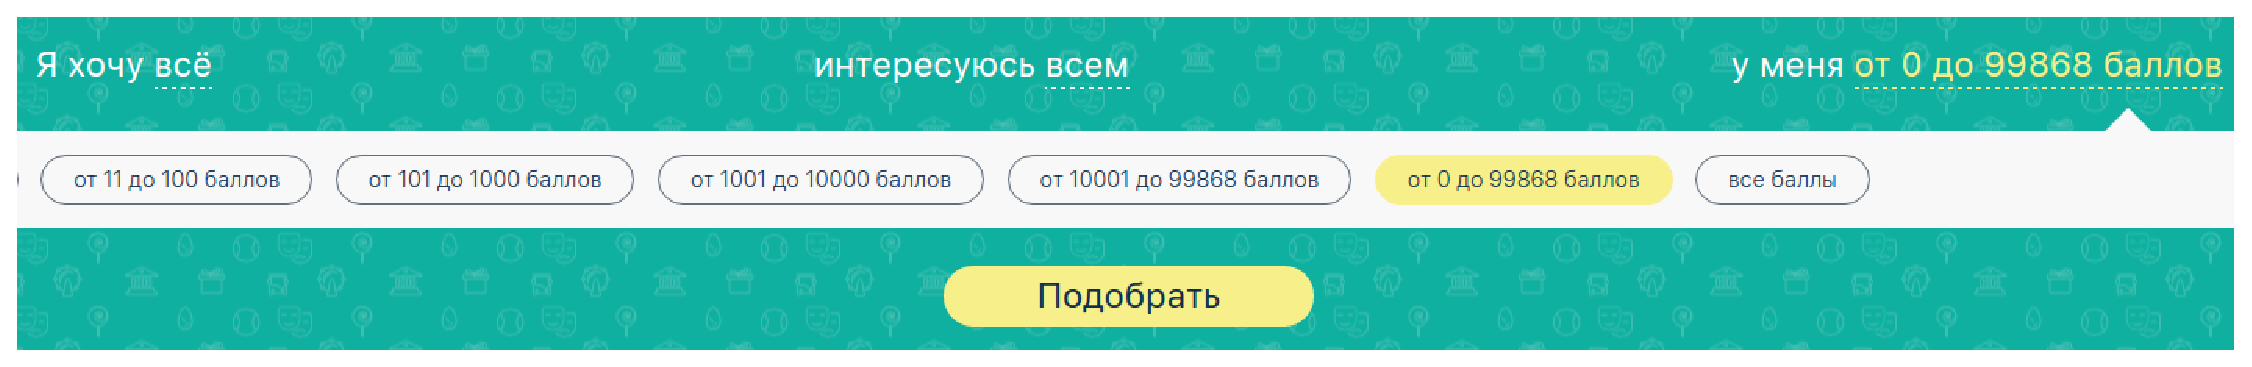
\includegraphics[width=170mm]{04_auth_funcs/figures/02.eps}
                \caption{Фильтр по количеству баллов}
                \label{fig:auth_filter}
            \end{figure}
        
        \subsection{Тизер товара}

            См. рис. \ref{fig:auth_tizer}
        
            Единственное отличие от тизера товара для неавторизованного 
            пользователя (см. \ref{sec:noauth_tizer})
            --- это активная ссылка <<желание>>.
            \begin{enumerate}
                \item Товар можно добавить в <<мои желания>> кликом по 
                <<сердечку>>
                \item Сердечко товара, добавленного в <<мои желания>> 
                заливается красным.
                \item Товар, добавленный в <<мои желания>> появляется в 
                соответствующем разделе (см.\ref{sec:auth_my_wishes}).
            \end{enumerate}

        
            \begin{figure}
                \center
                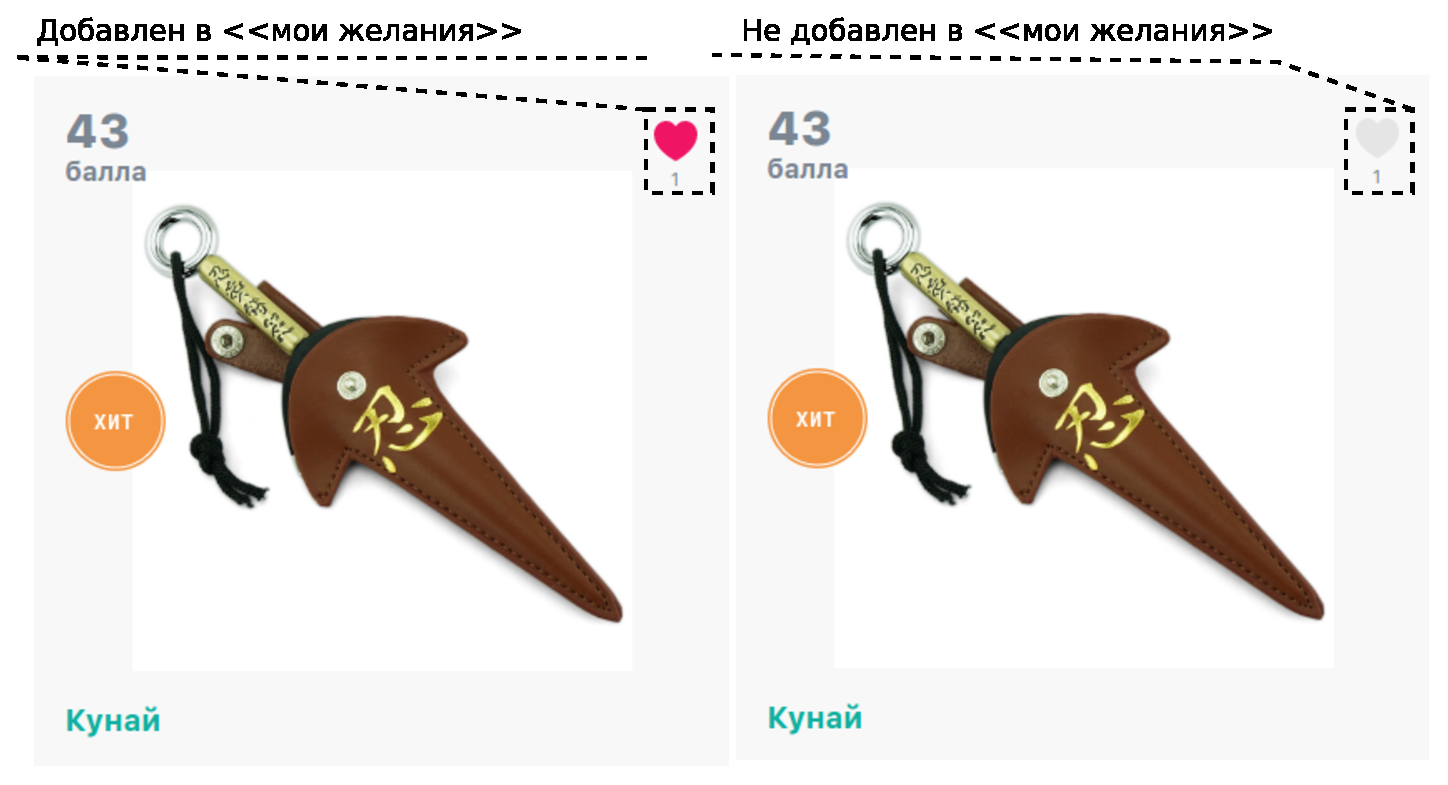
\includegraphics[width=170mm]{04_auth_funcs/figures/03.eps}
                \caption{Тизер товара для авторизованного пользователя.}
                \label{fig:auth_tizer}
            \end{figure}
        
        
    \section{Главная страница}
        \subsection{Банер-слайдер}
        
            См. рис. \ref{fig:auth_slide_goods}

            Единственное отличие от слайда-товара для неавторизованного 
            пользователя (см. \ref{sec:noauth_slide_goods})
            --- это активная ссылка <<желание>>.
            
            \begin{enumerate}
                \item Товар можно добавить в <<мои желания>> кликом по 
                <<сердечку>>
                \item Сердечко товара, добавленного в <<мои желания>> 
                заливается красным.
                \item Товар, добавленный в <<мои желания>> появляется в 
                соответствующем разделе (см.\ref{sec:auth_my_wishes}).
            \end{enumerate}
            
            \begin{figure}
                \center
                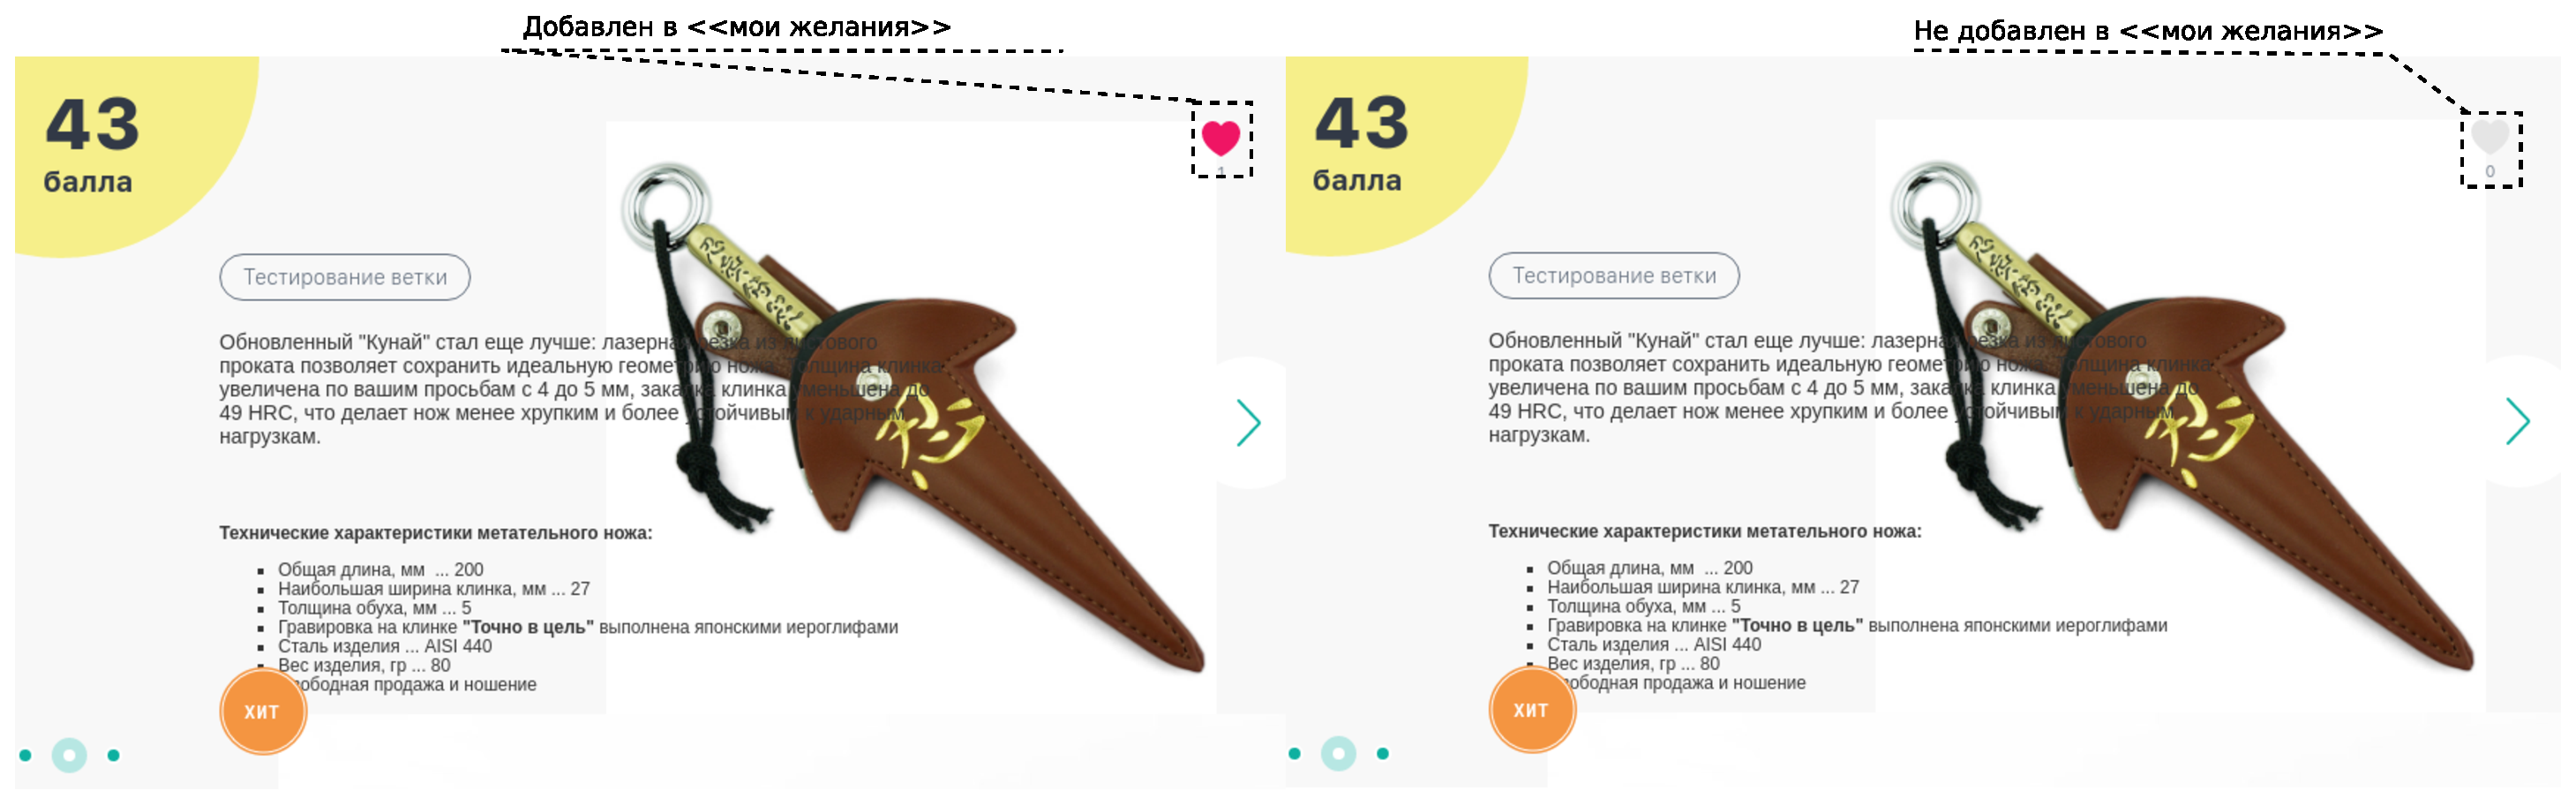
\includegraphics[width=170mm]{04_auth_funcs/figures/04.eps}
                \caption{Слайд-товар для авторизованного пользователя.}
                \label{fig:auth_slide_goods}
            \end{figure}
        
        
     \section{Карточка товара}

        См. рис. \ref{fig:auth_goods_cart}
            \begin{figure}
                \center
                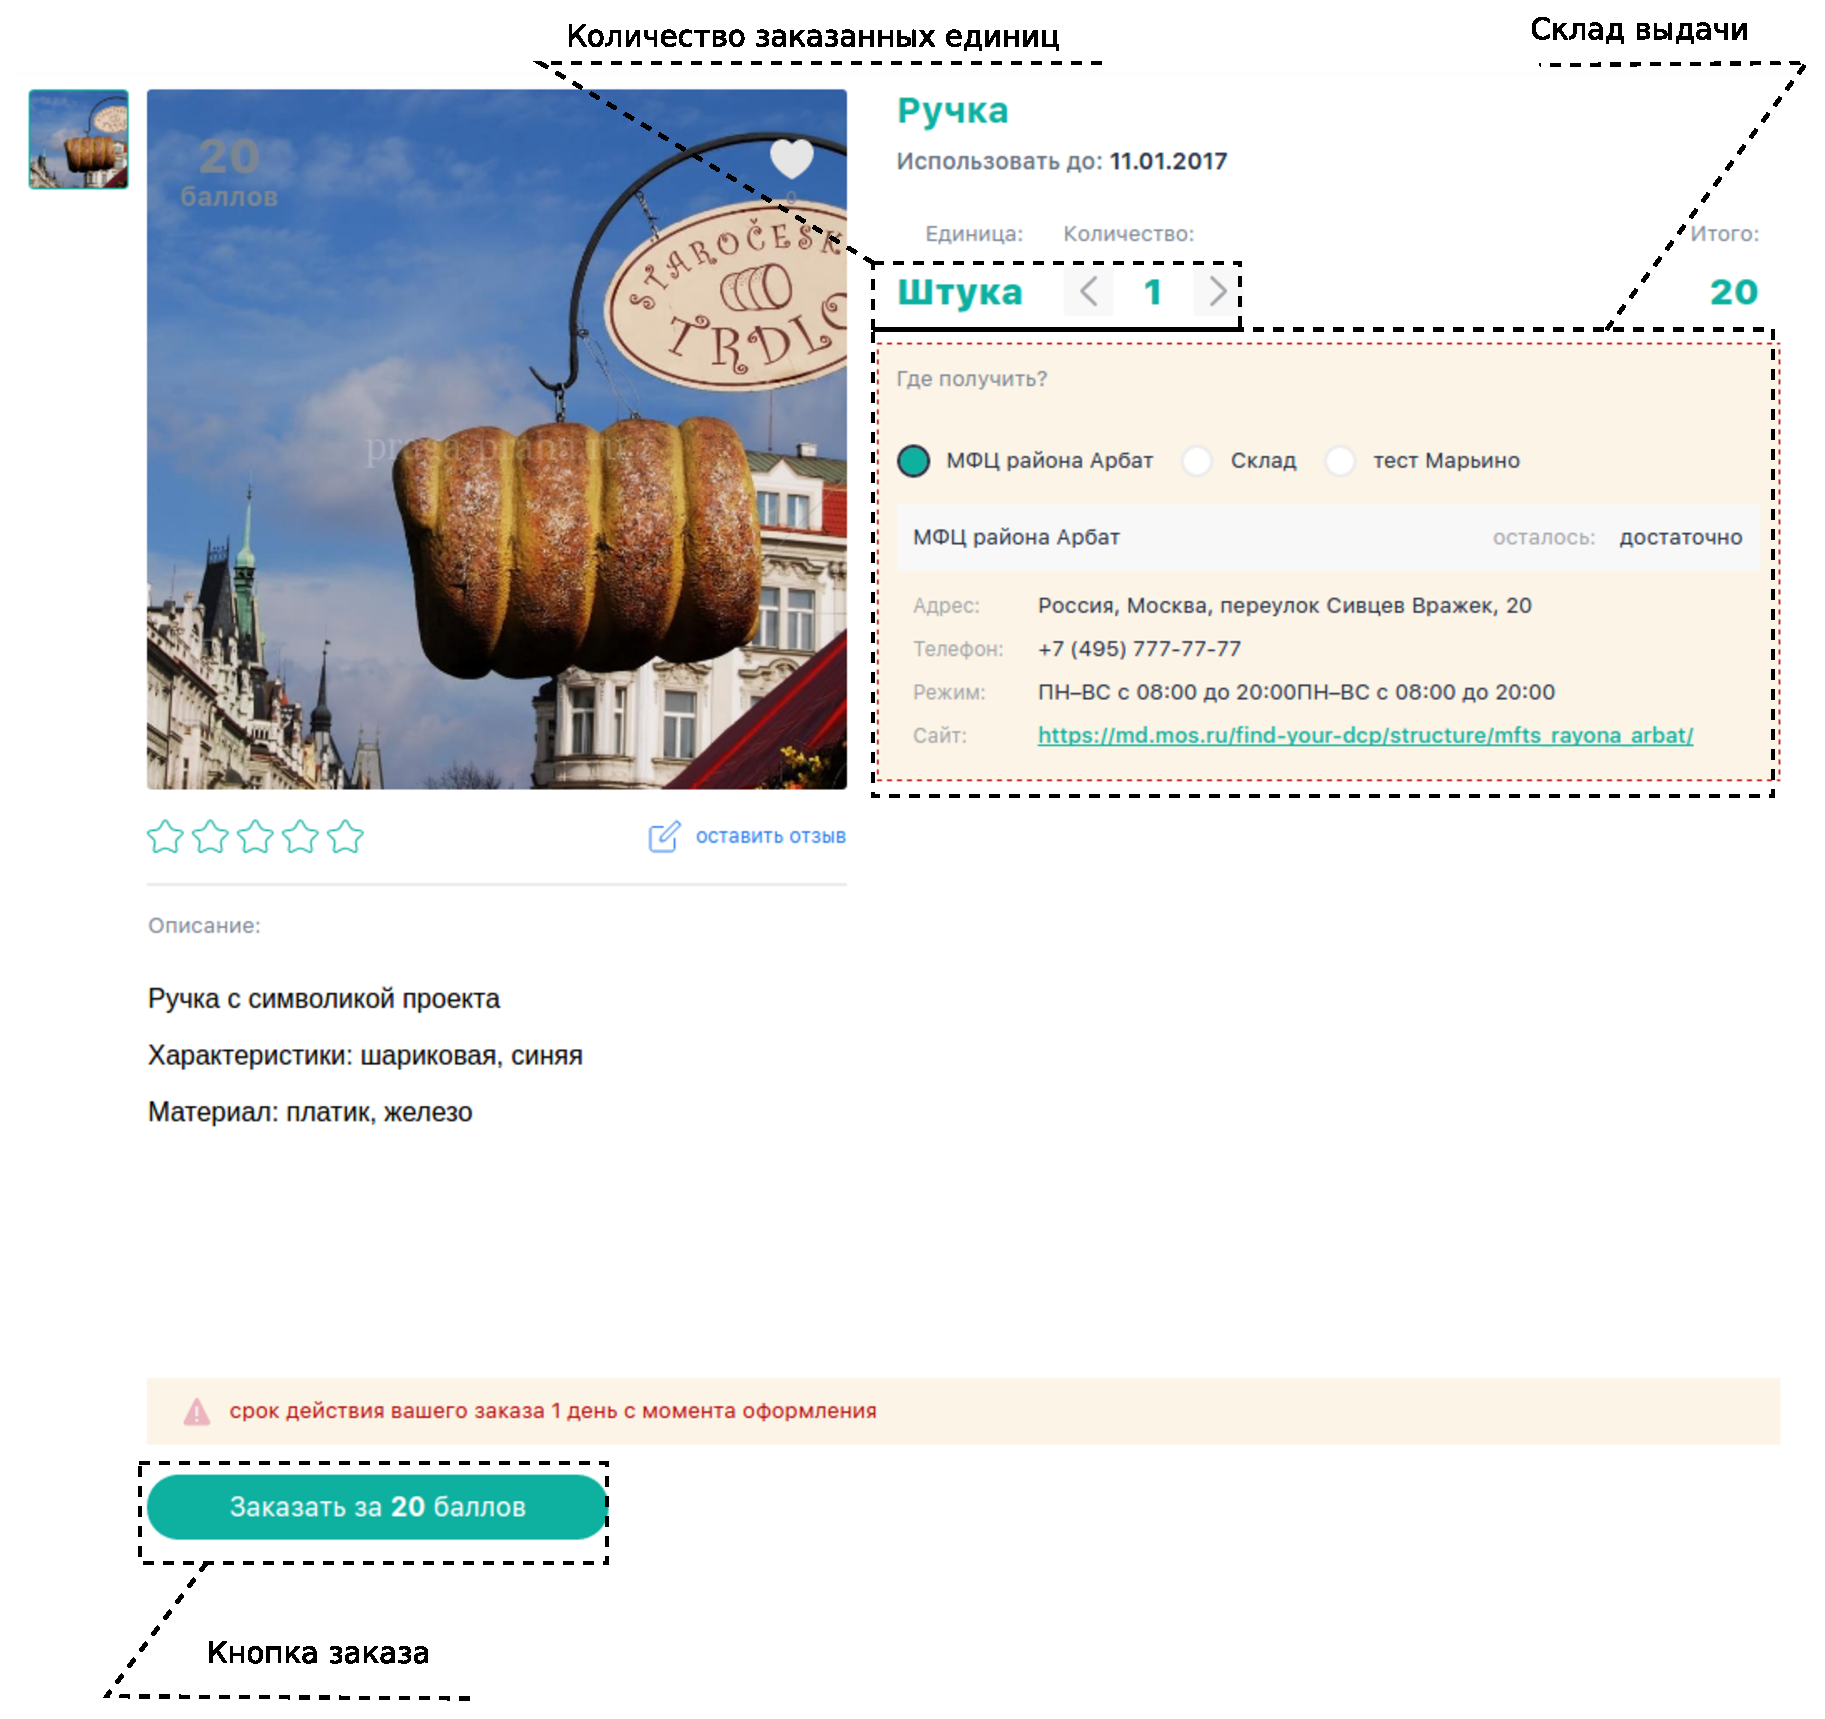
\includegraphics[width=170mm]{04_auth_funcs/figures/05.eps}
                \caption{Карточка товара для авторизованного пользователя}
                \label{fig:auth_goods_cart}
            \end{figure}
                
 
        Функционал карточки товаров для пользователя группы \gloss{auth_user}
        идентичен описанному в разделе \ref{sec:goods_cart}, за исключением
        появления и изменения нескольких элементов, описанных ниже.
     
        \subsection{Склад выдачи}\label{sec:auth_cart_store}

            Аналогичен \ref{sec:goods_cart_stores}, за исключением того, что 
            выбор конкретного склада при заказе будет означать получение 
            поощрения именно с него.

        \subsection{Количество заказываемых единиц}
            \begin{enumerate}
                \item По умолчанию для заказа установлен один \gloss{quant}.
                \item Количество заказываемых квантов поощрения не может быть
                больше доступных на выбранном(см.\ref{sec:auth_cart_store}) 
                складе
                \item При изменении количества заказываемых квантов
                автоматически пересчитывается общая сумма заказа в столбце <<ит
                ого>>.  \item Количество заказываемых квантов поощрения не 
                может быть больше, чем пользователь может себе позволить 
                исходя из имеющихся у него баллов.
            \end{enumerate}
            
        \subsection{Кнопка заказа}

            \begin{enumerate}
                \item Недоступна, если общая сумма заказа превышает количество
                имеющихся у пользователя баллов.
                \item На кнопке заказа отображается общая стоимость заказа и
                дублирует содержимое 
                \item При нажатии вызывается окно подтверждения заказа
                (см.\ref{sec:auth_cart_confirm}).
            \end{enumerate}

        \subsection{Форма подтверждения заказа}\label{sec:auth_cart_confirm}
            См. рис. \ref{fig:auth_cart_confirm}
            \begin{figure}
                \center
                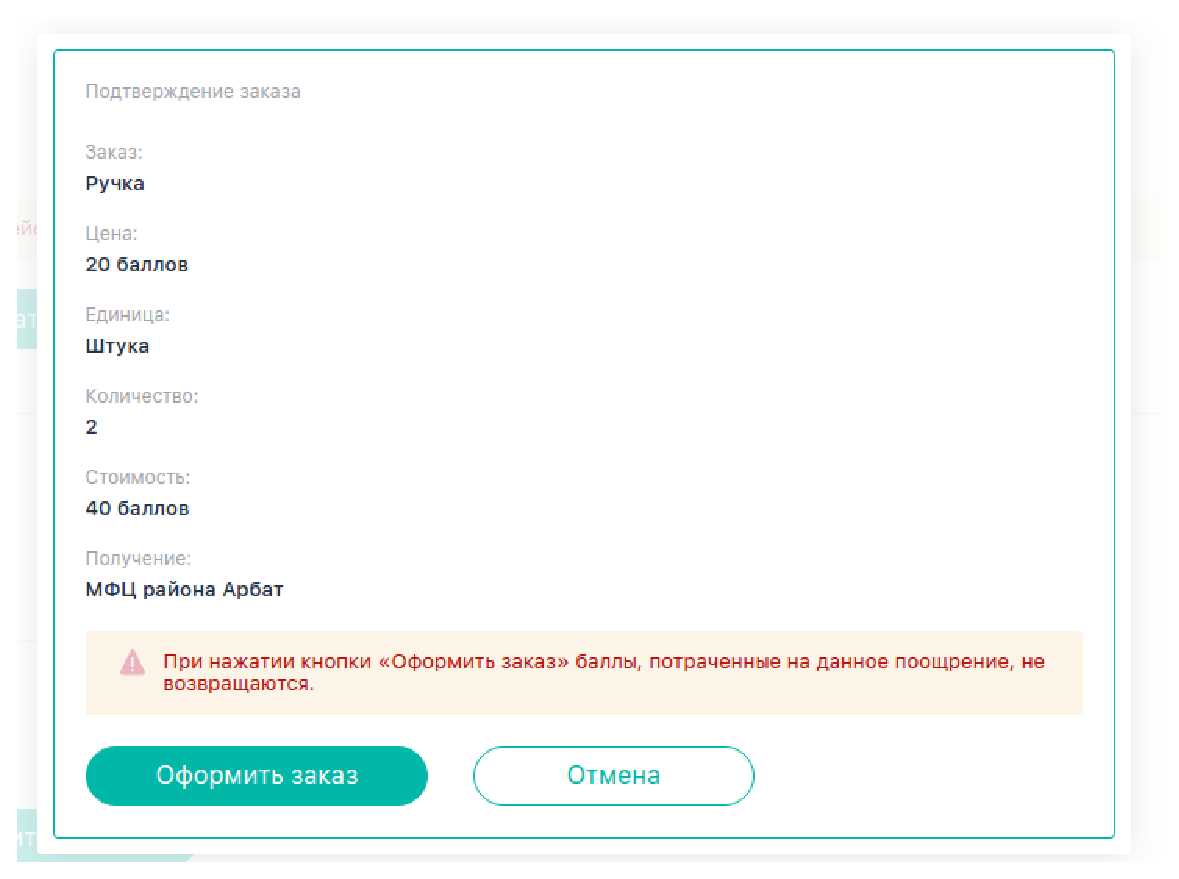
\includegraphics[width=100mm]{04_auth_funcs/figures/07.eps}
                \caption{Подтверждение заказа}
                \label{fig:auth_cart_confirm}
            \end{figure}
 
            Имеет следующие поля:

            \begin{enumerate}
                \item \textbf{заказ} --- наименование поощрения;
                \item \textbf{цена} -- цена одного кванта поощрения;
                \item \textbf{единица} --- см.\gloss{quant};
                \item \textbf{количество} -- количество квантов поощрения;
                \item \textbf{стоимость} -- общая стоимость заказа;
                \item \textbf{получение} -- \gloss{storage}, с которого
                необходимо будет забрать поощрение;
                \item сообщение о невозможности возвврата баллов, если отмена
                заказа для данного поощрения не предусмотрена.
            \end{enumerate}

            После успешного подтверждения заказа пользователя перенаправляет в
            раздел <<Мои заказы>> (см.\ref{sec:auth_my_orders}).

        \subsection{Отзывы}

            См. рис. \ref{fig:auth_goods_cart_otz}

            Отображение списка отзывов аналогично таковому у неавторизованного
            пользователя (см.\ref{sec:noauth_otz}), но появляется возможность 
            добавить свой отзыв через форму.

            \subsubsection{Форма добавления отзыва}
                
                \begin{enumerate}
                    \item Пользователь может добавить отзыв к товару только 
                    один раз
                    \item Пользователь может добавить отзыз, тлько если 
                    поставил оценку.
                \end{enumerate}

           \begin{figure}
                \center
                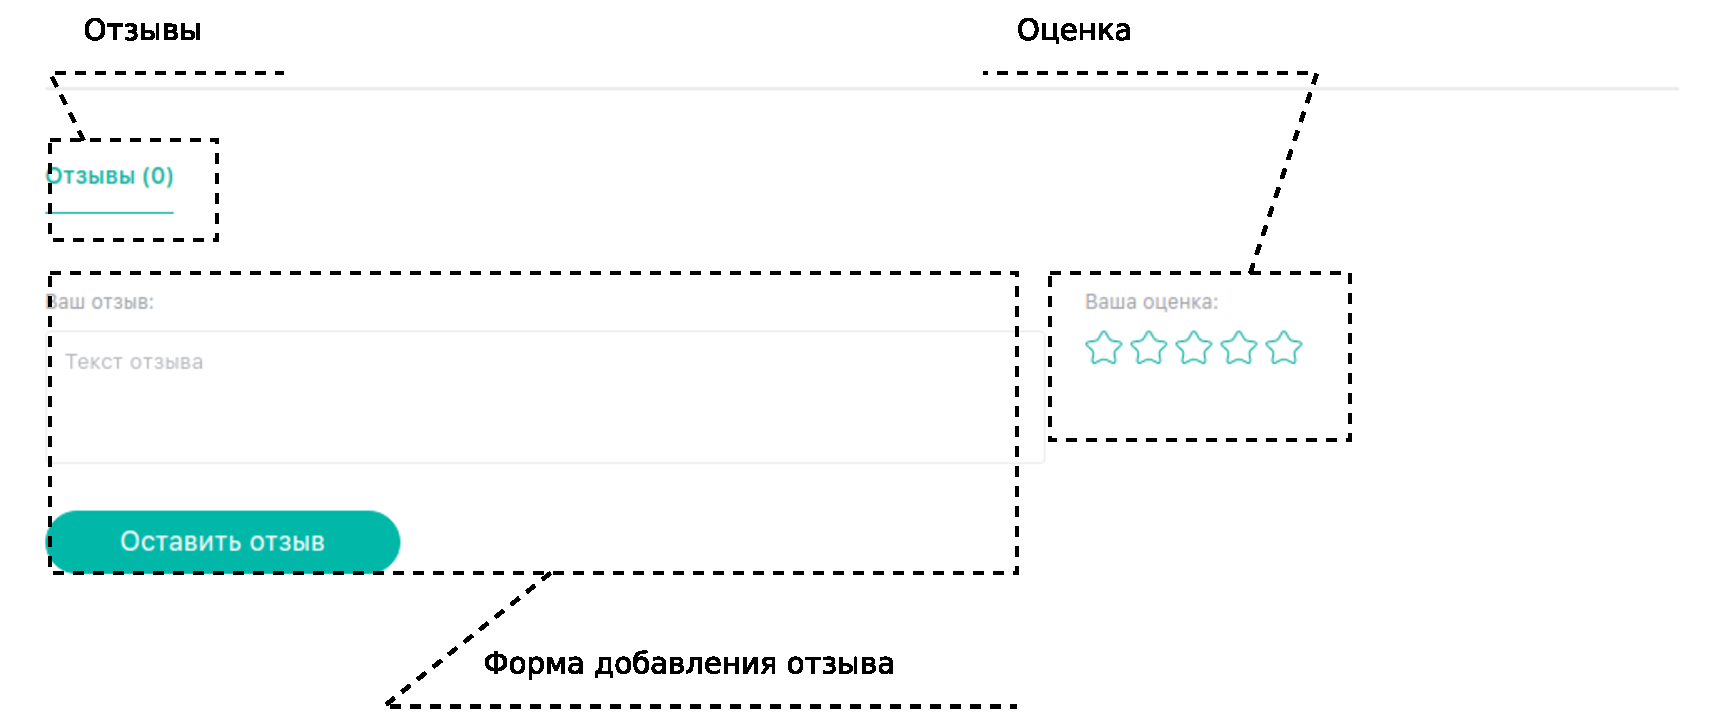
\includegraphics[width=170mm]{04_auth_funcs/figures/06.eps}
                \caption{Добавление отзыва для авторизованного пользователя}
                \label{fig:auth_goods_cart_otz}
            \end{figure}

               
     \section{Профиль пользователя}

        \subsection{Мои заказы}\label{sec:auth_my_orders}

            Данный раздел доступен только пользователю группы \gloss{auth_user}
            и содержит информацию о состоянии любого его заказа.

            \subsubsection{Статусы заказов}\label{sec:auth_order_statuses}
            
            \begin{itemize}
                \item \textbf{В работе} - заказ сделан через сайт и ожидает выдачи
                \item \textbf{Выполнен} - заказ выдан
                \item \textbf{Брак} - возврат заказа по причине брака
                \item \textbf{Отменен} - отмена заказа пользователем
                \item \textbf{Аннулирован} - отмена заказа за истечением срока получения
                (см. \ref{sec:goods_expires})

            \end{itemize}

            \subsubsection{Вкладка <<могу использовать>>}
            См рис. \ref{fig:auth_orders_may_use}

            В ней отображены заказы, находящеся в статусе <<В работе>> (см.
            \ref{sec:auth_order_statuses}).

            \begin{figure}
                \center
                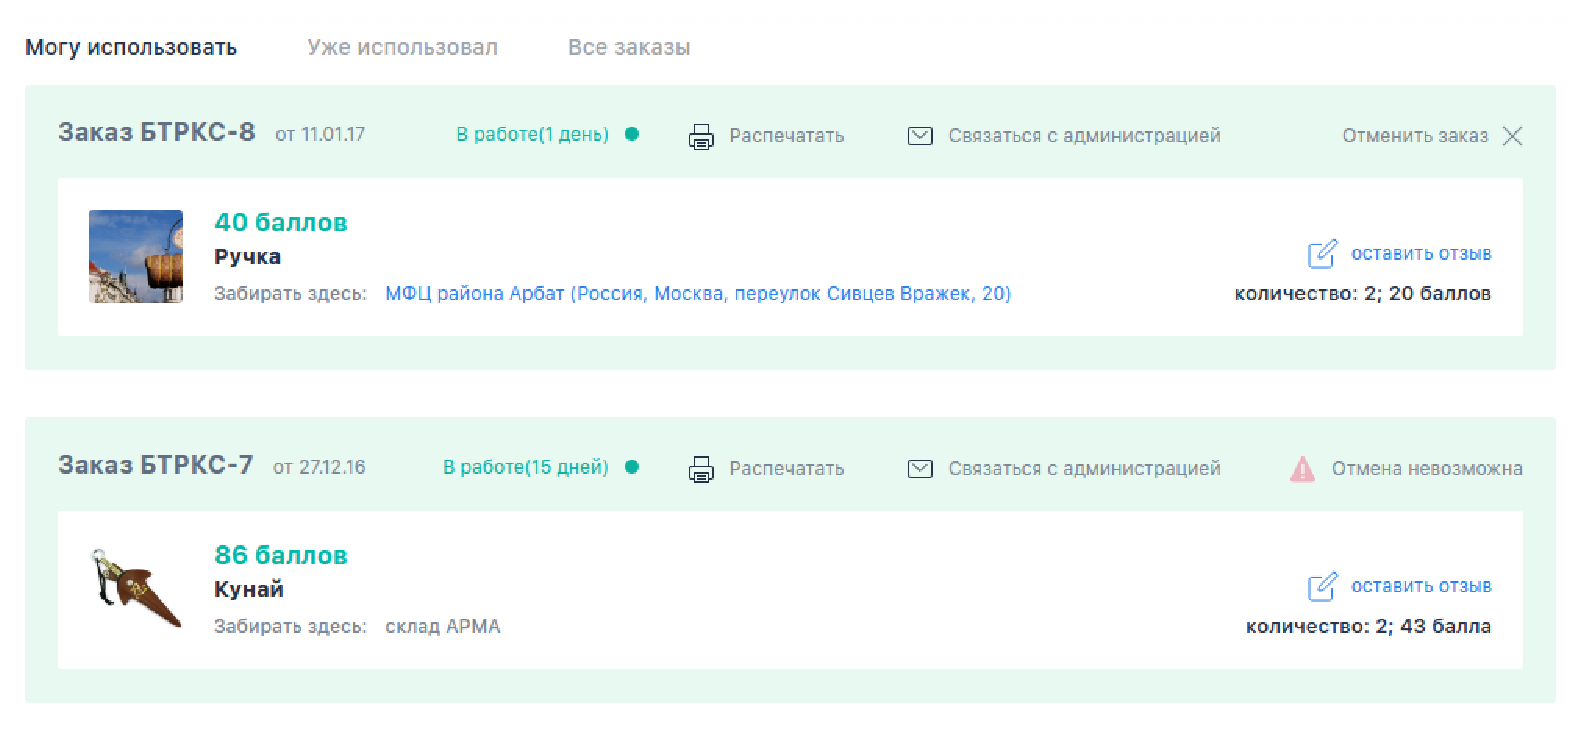
\includegraphics[width=100mm]{04_auth_funcs/figures/08.eps}
                \caption{Добавление отзыва для авторизованного пользователя}
                \label{fig:auth_orders_may_use}
            \end{figure}

            \subsubsection{Вкладка <<уже использовал>>}
            См рис. \ref{fig:auth_orders_already_use}

            В ней отображены заказы, находящеся в статусахе
            <<выполнен>>, <<брак>>, <<отменён>>, <<аннулирован>> (см.
            \ref{sec:auth_order_statuses}).

            \begin{figure}
                \center
                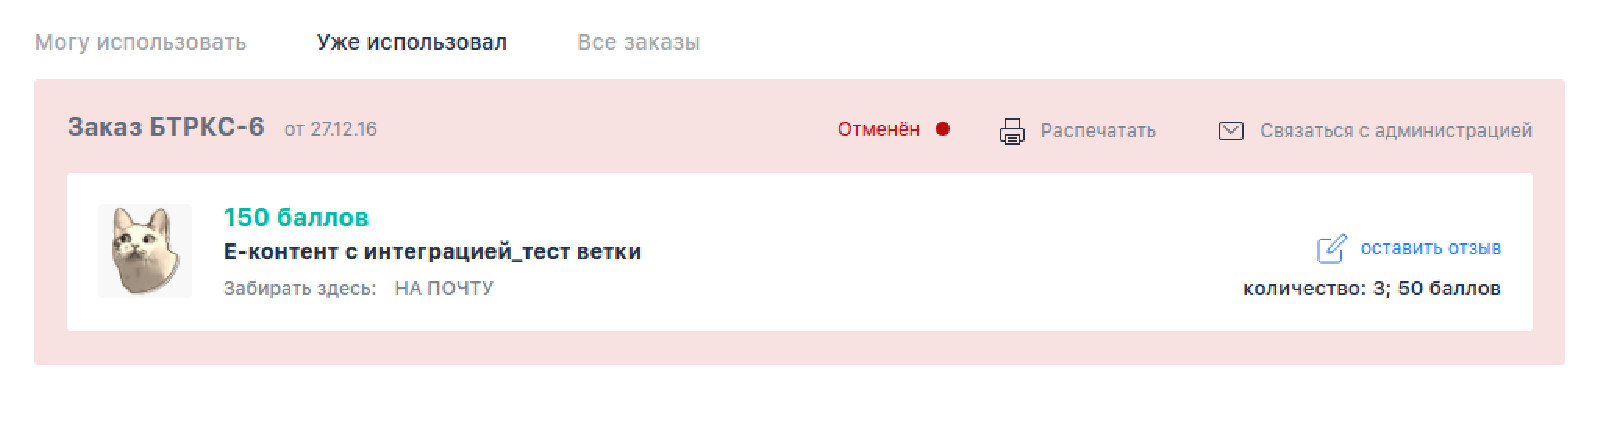
\includegraphics[width=100mm]{04_auth_funcs/figures/09.eps}
                \caption{Добавление отзыва для авторизованного пользователя}
                \label{fig:auth_orders_already_use}
            \end{figure}

            \subsubsection{Вкладка <<все заказы>>}
            См рис. \ref{fig:auth_orders_all_use}

            В этой вкладке отображаются все заказы во всех статусах
            (см. \ref{sec:auth_order_statuses})
            \begin{figure}
                \center
                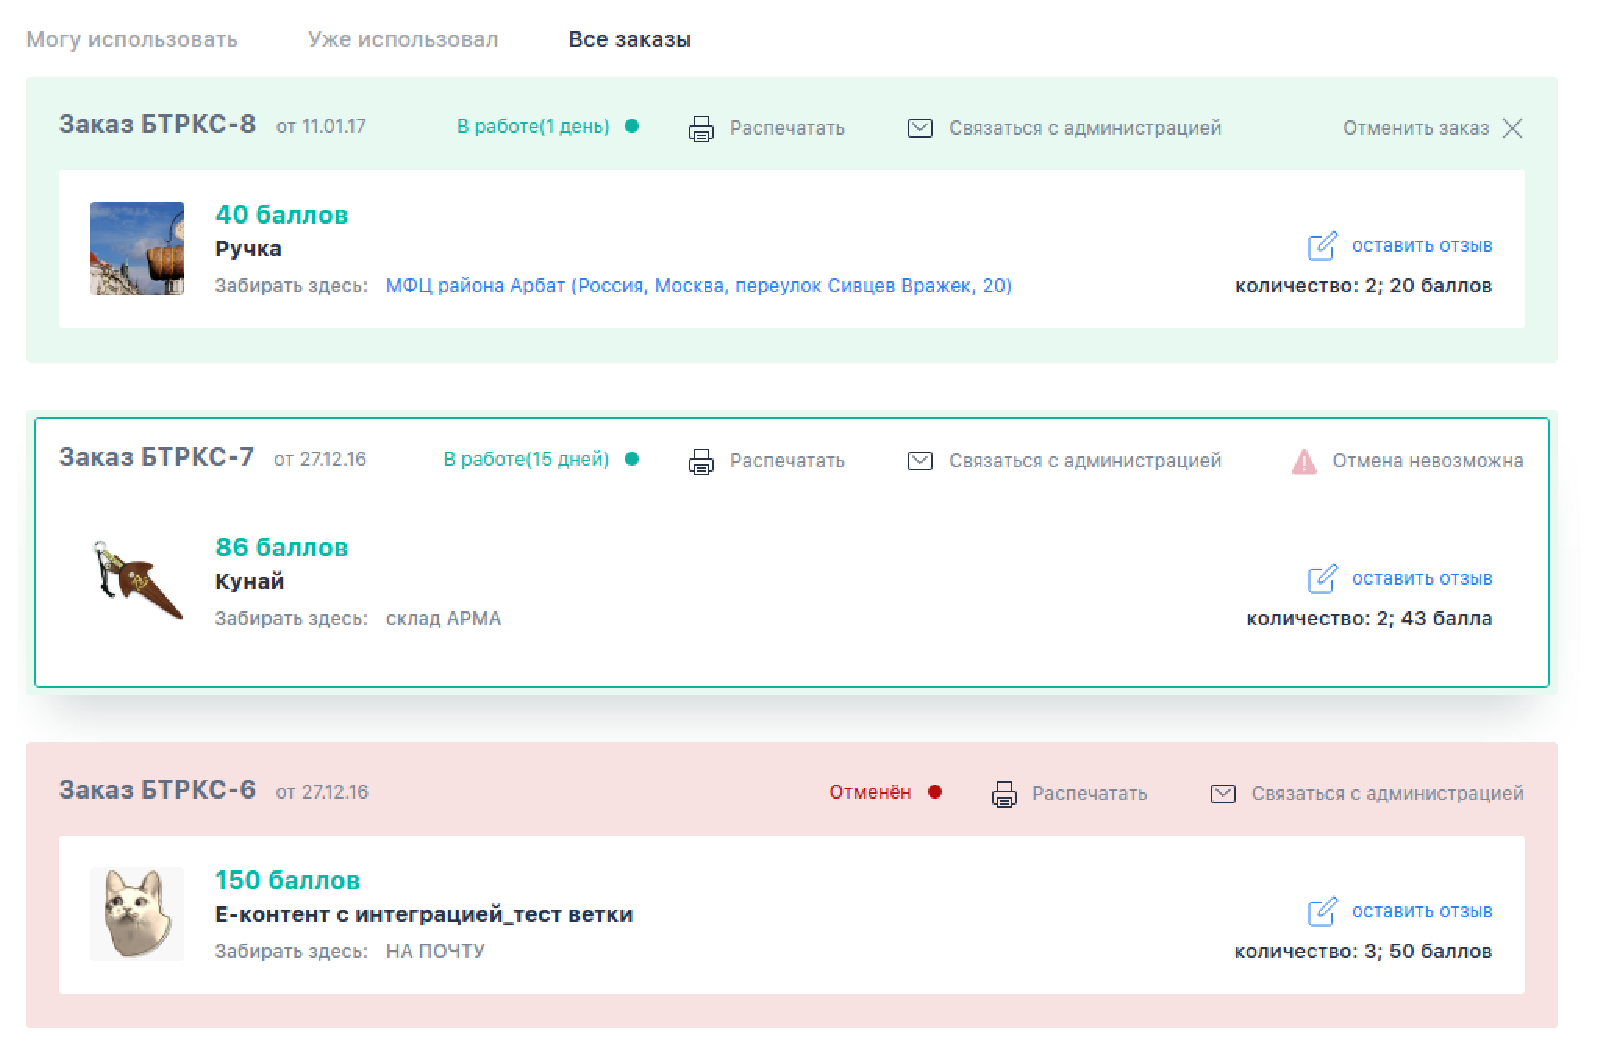
\includegraphics[width=100mm]{04_auth_funcs/figures/10.eps}
                \caption{Добавление отзыва для авторизованного пользователя}
                \label{fig:auth_orders_all_use}
            \end{figure}

            \subsubsection{Карточка заказа}

                См. рис. \ref{fig:auth_order_cart}

                \begin{figure}
                    \center
                    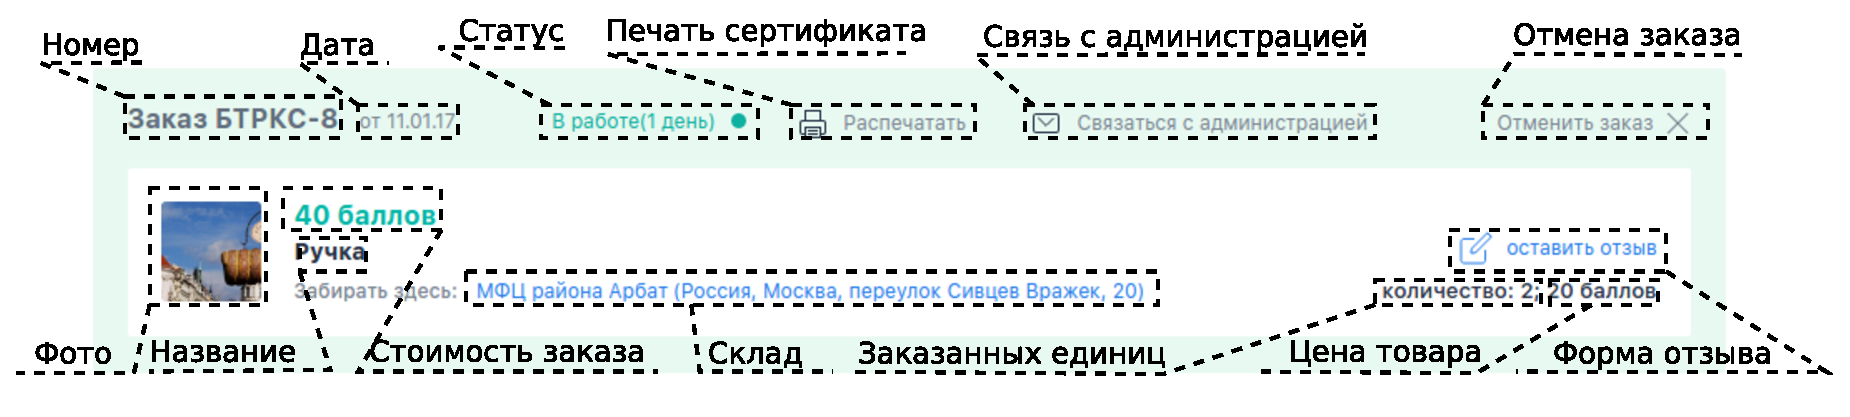
\includegraphics[width=170mm]{04_auth_funcs/figures/12.eps}
                    \caption{Добавление отзыва для авторизованного пользователя}
                    \label{fig:auth_order_cart}
                \end{figure}

                \paragraph{Номер заказа}
                    Сквозной номер заказа. Начинается с префикса <<БТРКС>>

                \paragraph{Дата заказа}
                    Дата, когда на сайте \gloss{shop} был сделан заказ

                \paragraph{Статус заказа}
                    Информация о текущем статусе и, для статуса <<в 
                    работе>>, о количестве дней, прошедших с момента заказа 
                    (см. \ref{sec:auth_order_statuses})

                \paragraph{Сертификат}
                См. рис. \ref{fig:auth_order_cert}

                \begin{enumerate}
                    \item Сертификат выдаётся на \gloss{nonmater_goods}.
                    \item Для \gloss{mater_goods} сертификат не доступен.
                    \item Сертификат содержит информацию, которую
                        \gloss{partner_ag} используют для предоставления
                        нематериальных поощрений.
                        \begin{itemize}
                            \item номер сертификата (формируется из номера
                            заказа);
                            \item срок действия;
                            \item ФИО лица, которому представляется поощрение;
                            \item наименование поощрения;
                            \item адрес, по которому расположен
                                \gloss{partner_ag};
                            \item правила предоставления поощрения;
                            \item карта-схема проезда;
                        \end{itemize}
                \end{enumerate}

                \begin{figure}
                    \center
                    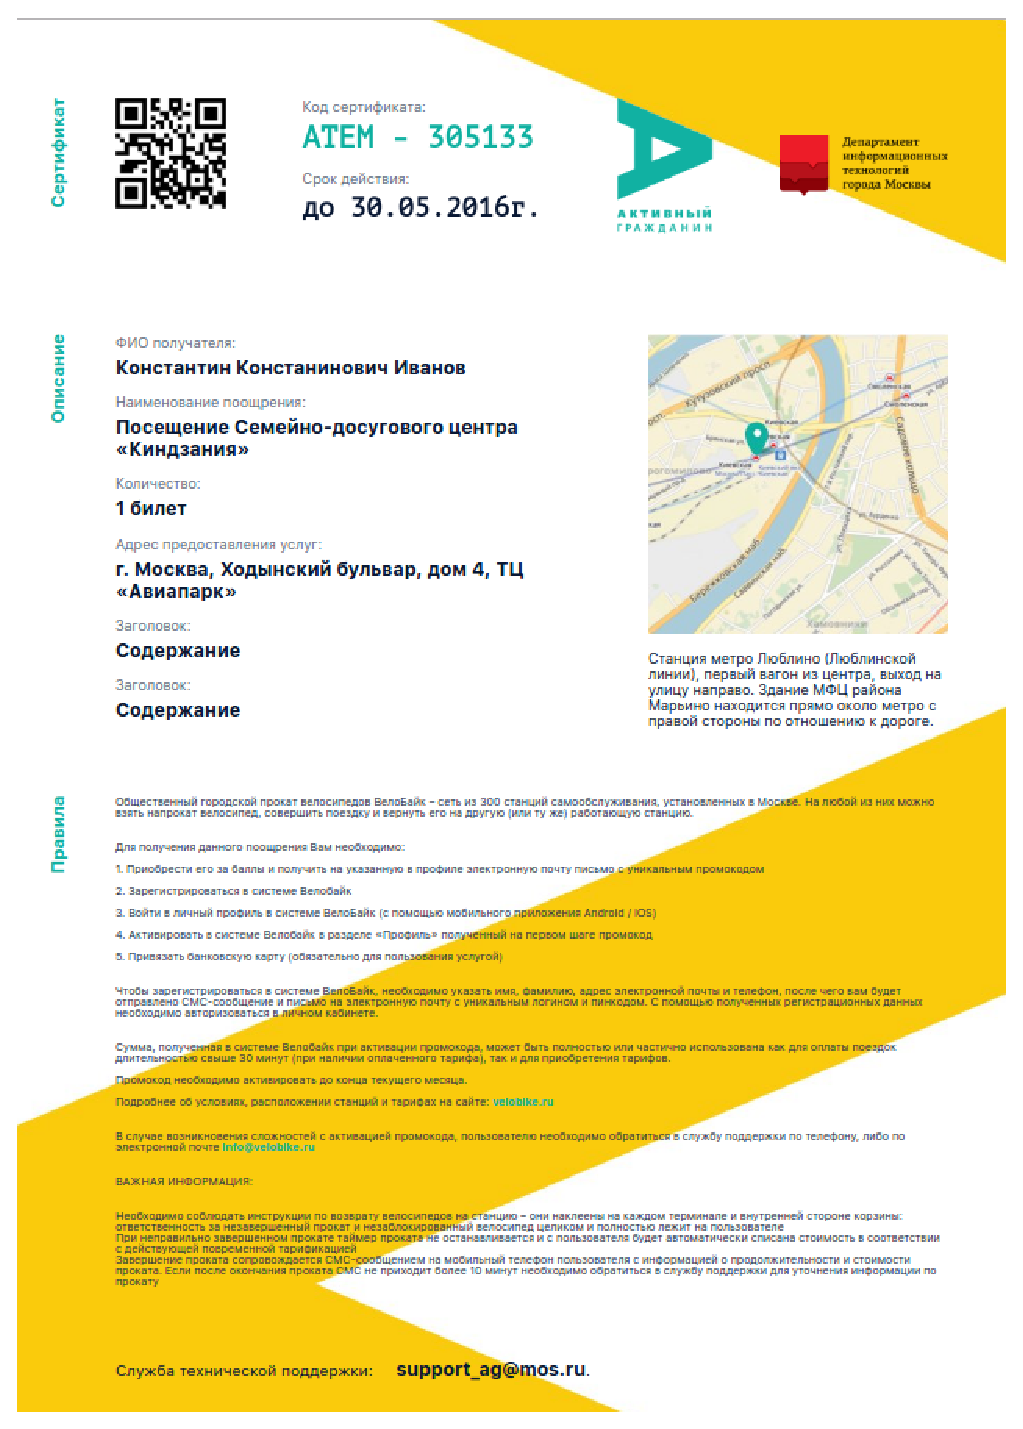
\includegraphics[width=120mm]{04_auth_funcs/figures/13.eps}
                    \caption{Сертификат.}
                    \label{fig:auth_order_cert}
                \end{figure}
 
                \paragraph{Связь с администрацией}
                См. рис. \ref{fig:auth_order_feedback}

                \begin{figure}
                    \center
                    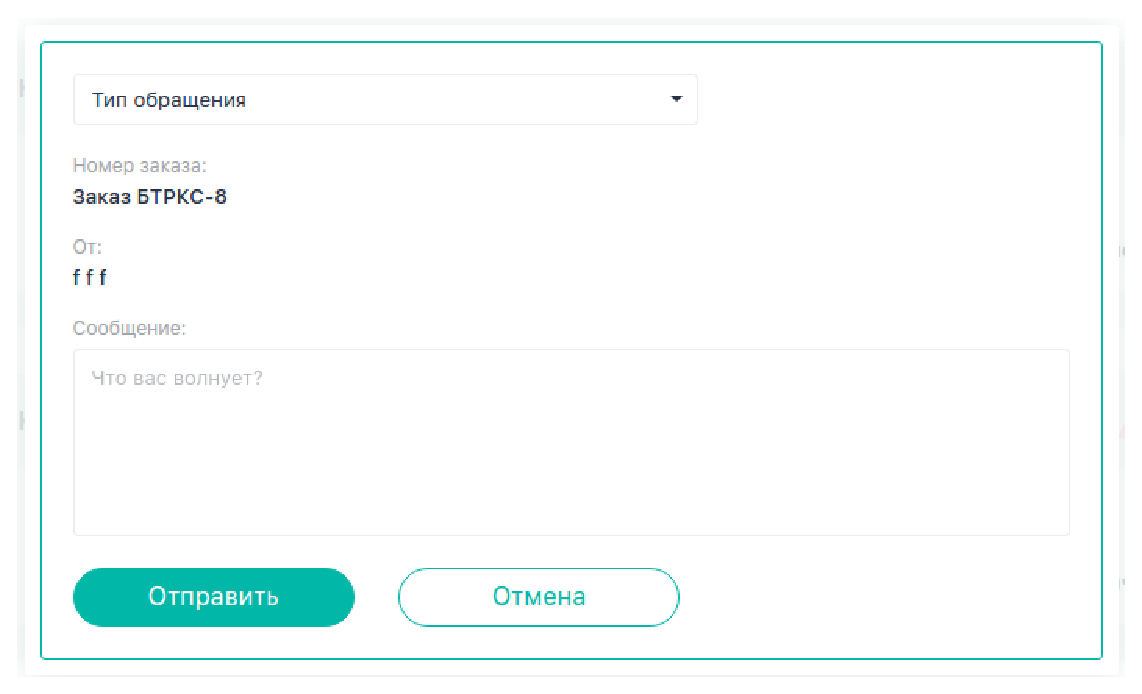
\includegraphics[width=120mm]{04_auth_funcs/figures/11.eps}
                    \caption{Связь с администрацией по поводу заказа.}
                    \label{fig:auth_order_feedback}
                \end{figure}
                \paragraph{Отмена заказа}
                \paragraph{Фото товара}
                \paragraph{Стоимость заказа}
                \paragraph{Название товара}
                \paragraph{Склад}
                \paragraph{Переход к форме отзыва}
                \paragraph{Количество заказанных единиц}
                \paragraph{Цена товара}
            
        \subsection{Мои баллы}

            См. рис. \ref{fig:auth_my_points}
        
            \subsubsection{Дата}
            \subsubsection{Операция}
            \subsubsection{Баллы}
            \subsubsection{Пагинация}
            
        \subsection{Мои желания}
            \label{sec:auth_my_wishes}
            См. рис. \ref{fig:auth_my_wishes}
        
        
        
